\clearpage
\title{Problem 4.3}
\author{}
\date{}
\maketitle

\section*{Problem Description}
Write a program that will prompt the user to enter a HEX digit character("0",......"9" or, "A",......"F"), display it on the next line in decimal, and ask the user if he or she wants to do it again. If the user types "Y" or "y", the program terminates. If the user enters an illegal character. prompt the user try again.

\section*{Process}
\subsection*{Code:}

\begin{multicols}{2}{ | }
    \begin{minted}[linenos,breaklines,breakanywhere]{nasm}
DATA SEGMENT
    CR EQU 0DH
    LF EQU 0AH
    MSG1 DB CR, LF, "Enter A HEX Digit: $"
    MSG2 DB CR, LF, "Do it again? $"
    MSG3 DB CR, LF, "In Decimal: $"
    MSG4 DB CR, LF, "In Decimal: 1$"
    MSG5 DB CR, LF, "Try Again.$"
    CHAR DB ?, '$'
    ANS DB ?, '$'
DATA ENDS 

CODE SEGMENT
    ASSUME CS:CODE, DS: DATA
    
START:
    MOV AX, DATA
    MOV DS, AX
    
LOOP_START:
    LEA DX, MSG1
    MOV AH, 9
    INT 21H
    
    MOV AH, 1
    INT 21H
    
    CMP AL, '0'
    JB NOT_NUM
    
    CMP AL, '9'
    JA NOT_NUM
    
    MOV ANS, AL
    
    LEA DX, MSG3
    MOV AH, 9
    INT 21H
    
    MOV DL, ANS
    MOV AH, 2
    INT 21H
    
    JMP LOOP_CHECK
    
NOT_NUM:
    CMP AL, 'A'
    JB ILLEGAL
    
    CMP AL, 'F'
    JA ILLEGAL
    
    MOV ANS, AL
    SUB ANS, 11H
    
    LEA DX, MSG4
    MOV AH, 9
    INT 21H
    
    MOV DL, ANS
    
    MOV AH, 2
    INT 21H
    JMP LOOP_CHECK
    
ILLEGAL:
    LEA DX, MSG5
    MOV AH, 9
    INT 21H
    
LOOP_CHECK:
    LEA DX, MSG2
    MOV AH, 9
    INT 21H
    
    MOV AH, 1
    INT 21H
    
    CMP AL, 'y'
    JZ LOOP_START
    
    CMP AL, 'Y'
    JZ LOOP_START
    
    MOV AH, 4CH
    INT 21H
    
CODE ENDS
END START
\end{minted}
\end{multicols}

\subsection*{Output}
\begin{center}
    \centering
    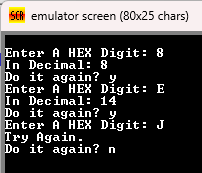
\includegraphics[width = .4\textwidth]{3.png}
    \captionof{figure}{Converting HEX to Decimal}
\end{center}
